\documentclass[aspectratio=169, 12pt]{beamer}

% Theme
\usetheme{metropolis}
\usepackage{booktabs}
\usepackage{colortbl}
\usepackage{xcolor}
\usepackage{graphicx}
\usepackage{tikz}
\usetikzlibrary{shapes.geometric, arrows.meta, positioning}
\usepackage{pgfplots}
\pgfplotsset{compat=1.18}
\usepackage{multirow}
\usepackage{array}

% ── Global spacing tightening ────────────────────────────────
\setlength{\parskip}{2pt}
\setbeamersize{text margin left=0.7cm, text margin right=0.7cm}
\setbeamertemplate{itemize/enumerate body begin}{\setlength\itemsep{2pt}\setlength\topsep{2pt}}
\setbeamertemplate{itemize/enumerate subbody begin}{\setlength\itemsep{1pt}}

% Colors
\definecolor{ulblue}{RGB}{0, 83, 154}
\definecolor{okgreen}{RGB}{0, 150, 80}
\definecolor{warnred}{RGB}{200, 40, 40}
\definecolor{warnorange}{RGB}{220, 120, 0}
\definecolor{lightgray}{RGB}{240, 240, 240}

\setbeamercolor{frametitle}{bg=ulblue, fg=white}
\setbeamercolor{progress bar}{fg=ulblue}
\setbeamercolor{alerted text}{fg=warnred}

% Macros
\newcommand{\good}[1]{\textcolor{okgreen}{\textbf{#1}}}
\newcommand{\bad}[1]{\textcolor{warnred}{\textbf{#1}}}
\newcommand{\warn}[1]{\textcolor{warnorange}{\textbf{#1}}}

% Metadata
\title{Deep Learning for Content Moderation\\on the Shareish Solidarity Platform}
\subtitle{Progress Report — Follow-up to October 2025}
\author{Seyfullah Ural\\[4pt]\small Supervisor: Raphaël Marée \quad Guest: Pierre Geurts}
\institute{University of Liège}
\date{April 2026}

% ─────────────────────────────────────────────────────────────
\begin{document}

\maketitle

% ─── BRIDGE: October → April ─────────────────────────────────
\begin{frame}[shrink=25]{Since October — What Changed}
  \small
  \begin{tabular}{p{0.42\textwidth} p{0.02\textwidth} p{0.46\textwidth}}
    \textbf{October 2025 — Open question} & & \textbf{April 2026 — Status} \\
    \midrule
    Which training approach? Option A (safety-specialized) vs B (general base model)
    & &
    \good{Resolved.} Option A — LlamaGuard-3-1B and ShieldGemma-2b evaluated as primary candidates \\[6pt]

    Two-tier architecture: ``possible approach under evaluation''
    & &
    \good{Confirmed.} Detoxify-M (Tier 1) + LoRA LG-1B (Tier 2), measured end-to-end \\[6pt]

    Evaluation framework: designed, not yet tested
    & &
    \good{Implemented.} 10 models × 8 datasets; extended with a \textbf{deployability axis} (VRAM, latency, energy) \\[6pt]

    French support: ``critical but underexplored''
    & &
    \good{Confirmed empirically.} EN→FR F1 gap up to $-$0.686 (KoalaAI); French is a hard constraint \\[6pt]

    LoRA fine-tuning on French data: planned
    & &
    \warn{Executed — partially.} FR-Hate Superset adapters increase precision (TNR $\uparrow$); Reddit-FR evaluation pending; domain closeness identified as a key variable for recall \\[6pt]

    Alan GPU cluster: ``to learn''
    & &
    \good{Operational.} Used for 48 h baseline run + LoRA training jobs \\
  \end{tabular}
\end{frame}

% ─── SLIDE 1: Context ────────────────────────────────────────
\begin{frame}[shrink=25]{Context: Shareish \& the Content Moderation Problem}
  \begin{columns}[T]
    \column{0.55\textwidth}
      \textbf{Shareish} — open-source platform for solidarity practices\\
      {\small mutual aid, generalized exchange, gift economy (ULiège)}
      \begin{itemize}
        \item Everything is free — no real or virtual currency
        \item Request or offer material, manual, intellectual,\\
              or logistical aid
        \item French-speaking community (Belgium/France)
        \item No dedicated moderation infrastructure\\
              \bad{user-reported harmful content goes unfiltered}
      \end{itemize}
      \vspace{4pt}
      \textbf{Problem:} Deploy an automated content moderator that is both
      \emph{accurate on French text} and \emph{feasible on NGO hardware}.

    \column{0.42\textwidth}
      \begin{block}{Thesis scope}
        \begin{itemize}
          \item Evaluate 10 pre-trained models on 8 datasets
          \item Primary axis: \textbf{French F1}
          \item Secondary axis: \textbf{Deployability}
          \item Fine-tune promising candidates (LoRA)
          \item Propose a production architecture
        \end{itemize}
      \end{block}
  \end{columns}
\end{frame}

% ─── SLIDE 2: Deployability framing ──────────────────────────
\begin{frame}[shrink=25]{The Deployability Axis — Why It Matters Here}
  \textit{\small\textcolor{gray}{Oct 2025: evaluation framework covered Technical, Legitimacy, Operational, Robustness, Impact — but VRAM and inference speed were not explicit hard constraints. This emerged as the central finding of Phase 1.}}\\[4pt]
  \begin{columns}[T]
    \column{0.48\textwidth}
      \small
      \textbf{Deployability metrics collected:}
      \begin{itemize}
        \item Peak GPU memory (MB) at inference
        \item Average inference latency (ms/sample)
        \item Energy consumption (kWh / run)
        \item CO$_2$ equivalent (kg)
      \end{itemize}
      \vspace{4pt}
      \textbf{Hardware tiers defined:}
      \begin{itemize}
        \item \good{CPU-only} — zero GPU requirement
        \item \good{$\leq$6 GB VRAM} — consumer GPU (RTX 3060)
        \item \warn{6–16 GB} — prosumer GPU
        \item \bad{$>$16 GB} — non-deployable for Shareish
      \end{itemize}

    \column{0.48\textwidth}
      \begin{alertblock}{Novel evaluation angle}
        \small
        Most NLP benchmarks rank models by accuracy alone.\\[4pt]
        \alert{A model requiring 24 GB VRAM does not exist as a deployment option for a small NGO.}\\[4pt]
        This thesis treats VRAM and latency as \emph{hard constraints}, not afterthoughts.
      \end{alertblock}
  \end{columns}
\end{frame}

% ─── SLIDE 3: Evaluation framework ──────────────────────────
\begin{frame}[shrink=25]{Proposed Evaluation Framework}
  \begin{columns}[T]
    \column{0.50\textwidth}
      \small\textbf{Primary development metric: F1 (macro)}\\[3pt]
      Consistent with 88\% of the literature; simple to compare across models and datasets.\\[5pt]

      \textbf{Imbalance correction: MCC}\\[3pt]
      Reddit-FR is class-imbalanced. F1 at a fixed threshold can be gamed by predicting the majority class. MCC accounts for all four cells of the confusion matrix without requiring a threshold sweep.\\[5pt]

      \textbf{Secondary (threshold-independent): AUC-PR}\\[3pt]
      AUC-ROC is misleading on imbalanced sets — FPR stays low when negatives are abundant. AUC-PR degrades visibly when the model makes false-positive errors, which is the critical failure mode for content moderation.

    \column{0.46\textwidth}
      \small\textbf{Reporting framework (5 dimensions):}
      \begin{enumerate}
        \item \textbf{Technical}: F1, MCC, AUC-PR per dataset
        \item \textbf{Robustness}: HateCheck pass rate (target $\geq$25/29)
        \item \textbf{Operational}: VRAM, latency (ms/sample), energy
        \item \textbf{Legitimacy}: FPR disparity across groups, consistency
        \item \textbf{Impact}: Human–AI agreement on Shareish data (Phase 3)
      \end{enumerate}
  \end{columns}
\end{frame}

% ─── SLIDE 4: Evaluation setup ───────────────────────────────
\begin{frame}[shrink=35]{Phase 1 — Evaluation Setup}
  \textit{\small\textcolor{gray}{Oct 2025: ``Option A (safety-specialized) vs B (general base model)?'' → Answered: we evaluated both tiers of Option A across 10 models.}}\\[4pt]
  \begin{columns}[T]
    \column{0.48\textwidth}
      \small\textbf{10 evaluated models:}\\[2pt]
      \begin{tabular}{ll}
        \toprule
        \textbf{Model} & \textbf{Tier} \\
        \midrule
        Detoxify-multilingual & CPU \\
        Detoxify-unbiased & CPU \\
        KoalaAI & CPU \\
        EthicalEye & CPU \\
        CitizenLab & CPU \\
        \midrule
        LlamaGuard-3-1B & 3 GB GPU \\
        ShieldGemma-2b & 5.7 GB GPU \\
        \midrule
        LlamaGuard-3-8B & 16 GB GPU \\
        ShieldGemma-9b & 18 GB GPU \\
        Mistral-7B & 14 GB GPU \\
        \bottomrule
      \end{tabular}

    \column{0.48\textwidth}
      \small\textbf{8 datasets:}
      \begin{itemize}
        \item \textbf{HateCheck-EN/FR} — functionality tests (counter-speech, slurs…)
        \item \textbf{FR-Hate Superset} — French hate speech corpus
        \item \textbf{ToxiGen} — LLM-generated implicit toxicity
        \item \textbf{OpenAI Moderation} — multi-category EN
        \item \textbf{Civil Comments} — Wikipedia talk-page toxicity
        \item \textbf{Reddit-EN / Reddit-FR} — social media, balanced
      \end{itemize}
      \vspace{3pt}
      \small\textbf{Protocol:} threshold 0.5 $\cdot$ \textbf{Primary metric:} HC-FR F1
  \end{columns}
\end{frame}

% ─── SLIDE 5: Phase 1 Key Findings ──────────────────────────
\begin{frame}[shrink=25]{Phase 1 — Key Findings}
  \begin{columns}[T]
    \column{0.48\textwidth}
      \textbf{What works:}
      \begin{itemize}
        \item[\good{$\checkmark$}] \textbf{Detoxify-M}: CPU, 6 ms, HC-FR 0.787, robust counter-speech
        \item[\good{$\checkmark$}] \textbf{LG-1B}: 3 GB, 33 ms, HC-FR 0.674 — improvable via fine-tuning
        \item[\good{$\checkmark$}] \textbf{SG-2b}: best raw FR F1 (0.858) but counter-speech flaw
      \end{itemize}
      \vspace{4pt}
      \textbf{What does not work:}
      \begin{itemize}
        \item[\bad{$\times$}] KoalaAI, Detoxify-unbiased: HC-FR F1 $\approx$ 0.10
        \item[\bad{$\times$}] All $>$6 GB models: ruled out by hardware constraint
      \end{itemize}

    \column{0.48\textwidth}
      \textbf{Methodological findings:}
      \begin{itemize}
        \item EN performance is not a reliable proxy for FR (gap up to $-0.686$)
        \item Inference bugs fixed in v1 → v3: ShieldGemma wrong generation method; KoalaAI argmax vs.\ sum of unsafe probabilities
        \item Checkpointing essential: full run took $\sim$48 h on Alan A5000
      \end{itemize}
      \vspace{4pt}
      \begin{block}{Conclusion of Phase 1}
        Two candidates selected for fine-tuning:\\
        \textbf{LG-1B} (primary) and \textbf{SG-2b} (secondary)
      \end{block}
  \end{columns}
\end{frame}

% ─── SLIDE 6: Phase 1 French results ─────────────────────────
\begin{frame}[shrink=25]{Phase 1 — French Performance Overview}
  \scriptsize
  \begin{table}
    \centering
    \begin{tabular}{lcccccc}
      \toprule
      \textbf{Model} & \textbf{HC-FR} & \textbf{RD-FR} & \textbf{FR-Hate} & \textbf{VRAM} & \textbf{ms/samp.} \\
      \midrule
      \rowcolor{lightgray}
      ShieldGemma-2b      & \good{0.858} & 0.311        & 0.648 & 5.7 GB      & 24 \\
      Detoxify-M          & \good{0.787} & \good{0.547} & 0.634 & CPU         & 6  \\
      LlamaGuard-3-1B     & 0.674        & 0.398        & 0.372 & 3.0 GB      & 33 \\
      EthicalEye          & 0.597        & —$^a$        & —$^a$ & CPU         & —$^a$ \\
      CitizenLab          & 0.541        & —$^a$        & —$^a$ & CPU         & —$^a$ \\
      \midrule
      \bad{KoalaAI}           & \bad{0.101} & —$^a$ & —$^a$ & CPU         & 8  \\
      \bad{Detoxify-unbiased} & \bad{0.101} & —$^a$ & —$^a$ & CPU         & 4  \\
      \midrule
      LlamaGuard-3-8B     & —$^b$        & —$^b$        & —$^b$ & \bad{16 GB} & — \\
      ShieldGemma-9b      & —$^b$        & —$^b$        & —$^b$ & \bad{18 GB} & — \\
      Mistral-7B          & —$^b$        & —$^b$        & —$^b$ & \bad{14 GB} & — \\
      \bottomrule
    \end{tabular}
  \end{table}
  \vspace{2pt}
  \scriptsize
  $^a$ Omitted: model eliminated at HC-FR; further evaluation not prioritised.
  \quad $^b$ Excluded by VRAM constraint ($>$6 GB); results exist but are not deployment-relevant.\\[3pt]
  \small\textbf{EN→FR gap:} KoalaAI HC-EN 0.787 vs HC-FR 0.101 ($\Delta = -0.686$) —
  EN performance is not a reliable proxy for French viability.
\end{frame}

% ─── SLIDE 6: Deployability analysis ─────────────────────────
\begin{frame}[shrink=25]{Phase 1 — Deployability vs.\ Accuracy Trade-off}
  \begin{columns}[T]
    \column{0.50\textwidth}
      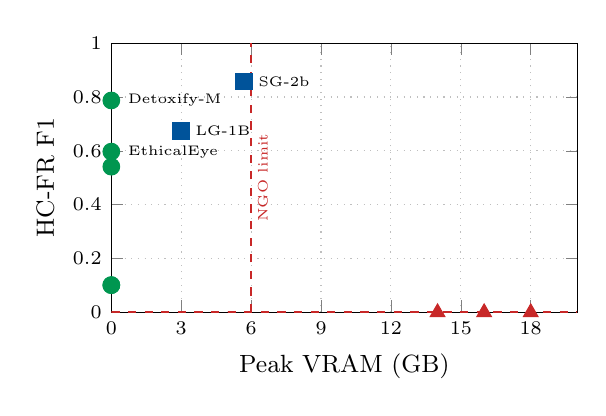
\begin{tikzpicture}
        \begin{axis}[
          width=7.5cm, height=5cm,
          xlabel={Peak VRAM (GB)},
          ylabel={HC-FR F1},
          xmin=0, xmax=20, ymin=0, ymax=1,
          xtick={0,3,6,9,12,15,18},
          ytick={0,0.2,0.4,0.6,0.8,1.0},
          grid=major, grid style={dotted, gray!50},
          tick label style={font=\scriptsize},
          label style={font=\small},
        ]
          \addplot[only marks, mark=*, mark size=3pt, color=okgreen]
            coordinates {(0,0.787)(0,0.101)(0,0.101)(0,0.597)(0,0.541)};
          \addplot[only marks, mark=square*, mark size=3pt, color=ulblue]
            coordinates {(3.0,0.674)(5.7,0.858)};
          \addplot[only marks, mark=triangle*, mark size=3pt, color=warnred]
            coordinates {(14,0)(16,0)(18,0)};
          \node[font=\tiny, anchor=west] at (axis cs:0.3,0.787) {Detoxify-M};
          \node[font=\tiny, anchor=west] at (axis cs:0.3,0.597) {EthicalEye};
          \node[font=\tiny, anchor=west] at (axis cs:3.2,0.674) {LG-1B};
          \node[font=\tiny, anchor=west] at (axis cs:5.9,0.858) {SG-2b};
          \addplot[dashed, thick, color=warnred, domain=0:20] {0};
          \draw[dashed, color=warnred, thick] (axis cs:6,0) -- (axis cs:6,1);
          \node[font=\tiny, color=warnred, rotate=90] at (axis cs:6.5,0.5) {NGO limit};
        \end{axis}
      \end{tikzpicture}

    \column{0.46\textwidth}
      \small\textbf{Findings:}
      \begin{itemize}
        \item Models $>$6 GB excluded by constraint alone
        \item \textbf{SG-2b} leads HC-FR (\good{0.858}, 5.7 GB, 24 ms)
        \item \textbf{Detoxify-M}: only competitive CPU option (\good{0.787}, 6 ms)
        \item Detoxify-M is $4\times$ faster than LG-1B
      \end{itemize}
      \vspace{4pt}
      \begin{block}{Efficiency frontier}
        \small Detoxify-M and LG-1B sit on the Pareto frontier of French F1 × VRAM × latency.
      \end{block}
  \end{columns}
\end{frame}

% ─── SLIDE 7: Counter-speech failure ─────────────────────────
\begin{frame}[shrink=25]{Phase 1 — HateCheck Functionality Breakdown}
  \textbf{HateCheck} tests 29 functional categories (slurs, derogation, counter-speech, spelling variants…)\\[4pt]
  \begin{columns}[T]
    \column{0.50\textwidth}
      \textbf{ShieldGemma-2b: counter-speech failure}\\[4pt]
      \small
      \begin{tabular}{lcc}
        \toprule
        \textbf{Category} & \textbf{SG-2b} & \textbf{Detoxify-M} \\
        \midrule
        \texttt{counter\_quote\_nh} & \bad{0.054} & \good{0.921} \\
        \texttt{counter\_ref\_nh}   & \bad{0.128} & \good{0.887} \\
        \midrule
        Hateful categories (avg)    & \good{0.91} & 0.74 \\
        \bottomrule
      \end{tabular}
      \vspace{4pt}

      Counter-speech quotes hateful language to rebut it.\\
      SG-2b classifies the quoted slur as the signal — \emph{correct-rate 5.4\%}.\\[4pt]
      \textbf{Deployment blocker}: users reporting content by quoting it would themselves be flagged.

    \column{0.46\textwidth}
      \textbf{Why it matters:}
      \begin{itemize}
        \item Aggregated F1 masks this failure (HC-FR F1 = 0.858 overall)
        \item Functionality-level breakdown is necessary for production safety
        \item Detoxify-M is robust to counter-speech despite lower overall F1
      \end{itemize}
      \vspace{6pt}
      \begin{alertblock}{Lesson}
        \small A high aggregate score does not certify fitness for deployment.
        Model selection must include targeted stress tests.
      \end{alertblock}
  \end{columns}
\end{frame}

% ─── SLIDE 9: Phase 2 LoRA setup ─────────────────────────────
\begin{frame}[shrink=25]{Phase 2 — LoRA Fine-Tuning Setup}
  \textit{\small\textcolor{gray}{Oct 2025: ``fine-tune on French datasets (10K–50K examples), then active learning with Shareish data'' → executed as LoRA on FR-Hate Superset + Reddit-FR.}}\\[4pt]
  \begin{columns}[T]
    \column{0.48\textwidth}
      \textbf{Why LoRA (Low-Rank Adaptation)?}
      \begin{itemize}
        \item Full fine-tuning of LG-1B / SG-2b requires 16–40 GB VRAM
        \item LoRA injects trainable low-rank adapters into attention layers
        \item Reduces training VRAM to $\sim$6–8 GB — fits A5000 (24 GB)
        \item Adapter size: $\sim$10 MB vs.\ full checkpoint ($\sim$4 GB)
      \end{itemize}

    \column{0.48\textwidth}
      \textbf{Configuration:}\\[4pt]
      \small
      \begin{tabular}{ll}
        \toprule
        Rank $r$ & 16 \\
        Alpha $\alpha$ & 32 \\
        Learning rate & $2 \times 10^{-4}$ \\
        Epochs & 3 (best = epoch 1) \\
        Batch size & 8 \\
        GPU & NVIDIA A5000 (24 GB) \\
        \bottomrule
      \end{tabular}
  \end{columns}
  \vspace{6pt}
  \textbf{Training data:} FR-Hate Superset + Reddit-FR \quad
  \textbf{Models:} LlamaGuard-3-1B, ShieldGemma-2b\\
  \textbf{Hypothesis:} Joint training covers both formal and informal French hate speech styles.
\end{frame}

% ─── SLIDE 10: Phase 2 experiments ───────────────────────────
\begin{frame}[shrink=25]{Phase 2 — LoRA Fine-Tuning Experiments}
  \begin{columns}[T]
    \column{0.52\textwidth}
      \textbf{Experiment 1 — Separate adapters on FR-Hate Superset}\\
      \small 20\% held-out test set, no overlap with training data.\\[4pt]
      \scriptsize
      \begin{tabular}{llcccc}
        \toprule
        \textbf{Model} & & \textbf{F1} & \textbf{Prec.} & \textbf{TPR} & \textbf{TNR} \\
        \midrule
        \multirow{2}{*}{LG-1B}
          & Baseline & 0.371 & 0.285 & 0.532 & 0.591 \\
          & LoRA     & \good{0.557} & \good{0.640} & 0.493 & \good{0.915} \\
        \midrule
        \multirow{2}{*}{SG-2b}
          & Baseline & 0.413 & 0.405 & 0.420 & 0.811 \\
          & LoRA     & \good{0.534} & \good{0.758} & 0.413 & \good{0.960} \\
        \bottomrule
      \end{tabular}
      \vspace{4pt}
      \small \good{F1 improves for both models.}\\
      Gain is \textbf{precision-driven} (TNR $\uparrow\uparrow$, TPR $\approx$ flat).\\
      Models learn what is \emph{not} harmful — not what \emph{is}.

    \column{0.44\textwidth}
      \textbf{Experiment 2 — Reddit-FR adapter \warn{(pending)}}\\
      \small
      \begin{itemize}
        \item LG-1B adapter exists — fair eval not yet submitted
        \item SG-2b training failed (SLURM timeout) — needs resubmit with \texttt{-{}-epochs 1}
        \item Contaminated run showed severe TPR collapse ($0.298 \to 0.089$) — fair eval will clarify
      \end{itemize}
      \vspace{5pt}
      \begin{block}{Next experiment — Joint training}
        \small Train one adapter on FR-Hate + Reddit-FR simultaneously.\\[3pt]
        \textbf{Hypothesis:} combined signal may force generalisation across formal and informal registers.\\[3pt]
        Requires a proper held-out eval from the start.
      \end{block}
  \end{columns}
\end{frame}

% ─── SLIDE 11: Domain closeness → Data Collection ────────────
\begin{frame}[shrink=25]{Phase 2 — Domain Closeness \& Data Collection}
  \begin{columns}[T]
    \column{0.50\textwidth}
      \textbf{Why publicly available data is insufficient}\\[4pt]
      \small
      Training corpora are \emph{domain-distant} from real Shareish content:
      \begin{itemize}
        \item FR-Hate Superset: formal academic sentences, explicit slurs
        \item Reddit-FR: informal text, irony, noisy community labels
        \item Shareish: solidarity context, Belgian French, community-specific norms
      \end{itemize}
      \vspace{4pt}
      Fine-tuning on formal hate corpora teaches models which \emph{known patterns} are not harmful (precision $\uparrow$), but cannot generalise to unseen platform-specific content.\\[4pt]
      \textbf{Hypothesis:} data from platforms with similar distributions to Shareish should transfer better.

    \column{0.46\textwidth}
      \begin{block}{Data Collection — Phase 3}
        \small
        Shareish data would be ideal — but there is not enough available data.\\[4pt]
        \textbf{Strategy:} collect from solidarity and exchange platforms with similar content distributions:
        \begin{itemize}
          \item Facebook solidarity groups
          \item Commercial exchange groups
          \item Vinted, donnons.org
        \end{itemize}
      \end{block}
      \vspace{4pt}
      \begin{alertblock}{\small Disclaimer — data sourcing}
        \small Scraping external platforms is \textbf{prohibited by Terms of Use} and raises \textbf{GDPR concerns}.
        Must use licensed corpora or explicit user consent.
      \end{alertblock}
  \end{columns}
\end{frame}

% ─── SLIDE 12: Architecture recommendation ───────────────────
\begin{frame}[shrink=25]{Recommendation — Two-Tier Production Architecture}
  \textit{\small\textcolor{gray}{Oct 2025: ``possible two-tier hybrid — Detoxify pre-filter + Llama Guard for complex cases (under evaluation)'' → now a concrete recommendation backed by Phase 1 \& 2 numbers.}}\\[4pt]
  \begin{columns}[T]
    \column{0.52\textwidth}
      \scalebox{0.78}{%
      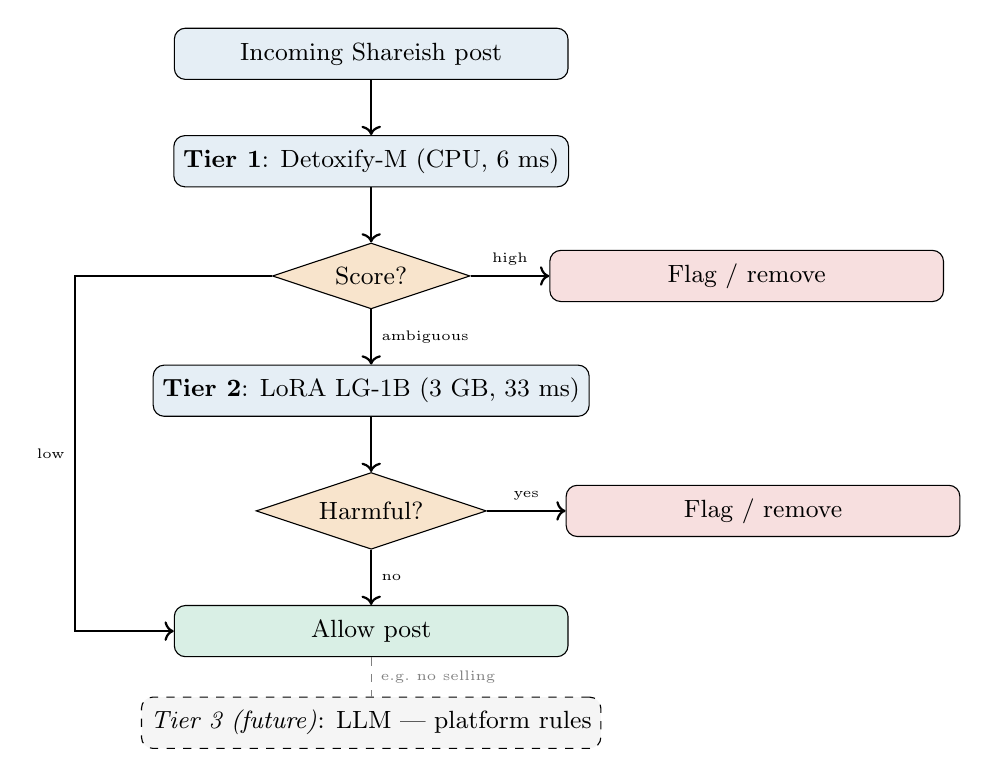
\begin{tikzpicture}[
        node distance=0.7cm,
        box/.style={draw, rounded corners, fill=ulblue!10, minimum width=5cm, minimum height=0.65cm,
                    font=\small, align=center},
        decision/.style={draw, diamond, fill=warnorange!20, font=\small, align=center, aspect=3},
        arrow/.style={->, thick}
      ]
        \node[box] (input) {Incoming Shareish post};
        \node[box, below=of input] (tier1) {\textbf{Tier 1}: Detoxify-M (CPU, 6 ms)};
        \node[decision, below=of tier1] (dec1) {Score?};
        \node[box, right=1.0cm of dec1, fill=warnred!15] (block) {Flag / remove};
        \node[box, below=of dec1] (tier2) {\textbf{Tier 2}: LoRA LG-1B (3 GB, 33 ms)};
        \node[decision, below=of tier2] (dec2) {Harmful?};
        \node[box, right=1.0cm of dec2, fill=warnred!15] (block2) {Flag / remove};
        \node[box, below=of dec2, fill=okgreen!15] (allow) {Allow post};
        \node[draw, dashed, rounded corners, fill=gray!8, below=0.5cm of allow,
              minimum width=5cm, minimum height=0.65cm, font=\small, align=center]
              (tier3) {\textit{Tier 3 (future)}: LLM — platform rules};
        \draw[arrow] (input) -- (tier1);
        \draw[arrow] (tier1) -- (dec1);
        \draw[arrow] (dec1) -- node[above, font=\tiny]{high} (block);
        \draw[arrow] (dec1) -- node[right, font=\tiny]{ambiguous} (tier2);
        \draw[arrow] (dec1.west) -- ++(-2.5,0) |-
              node[left, font=\tiny, pos=0.25]{low} (allow.west);
        \draw[arrow] (tier2) -- (dec2);
        \draw[arrow] (dec2) -- node[above, font=\tiny]{yes} (block2);
        \draw[arrow] (dec2) -- node[right, font=\tiny]{no} (allow);
        \draw[dashed, gray] (allow) -- node[right, font=\tiny, color=gray]{e.g.\ no selling} (tier3);
      \end{tikzpicture}%
      }

    \column{0.44\textwidth}
      \small
      \textbf{CPU-only:} Detoxify-M alone\\
      HC-FR 0.787, 6 ms, zero GPU.\\[5pt]

      \textbf{With 3–6 GB GPU:} two-tier\\
      Tier 1 routes on score: high → flag,\\
      low → allow (never reaches Tier 2),\\
      ambiguous → Tier 2.\\[5pt]

      \textbf{Advantages:}
      \begin{itemize}
        \item Counter-speech protected end-to-end
        \item Tier 2 only sees genuinely ambiguous content
        \item Combined latency $\leq$39 ms
      \end{itemize}
  \end{columns}
\end{frame}

% ─── SLIDE 13: Phase 3 plan ──────────────────────────────────
\begin{frame}[shrink=25]{Phase 3 — Next Steps}
  \begin{columns}[T]
    \column{0.48\textwidth}
      \textbf{Data Collection (primary focus):}
      \begin{enumerate}
        \item \textbf{Source domain-close data}: collect from solidarity and exchange platforms (Facebook groups, donnons.org, Vinted…)
        \item \textbf{Annotation}: label for harmful content with platform-specific patterns in mind
        \item \textbf{Synthetic augmentation}: AI-generated examples matching platform register
      \end{enumerate}
      \vspace{3pt}
      \scriptsize\textit{Terms of Use and GDPR compliance must be addressed before any scraping.
      }\normalsize

    \column{0.48\textwidth}
      \textbf{Fine-tuning \& evaluation:}
      \begin{enumerate}
        \setcounter{enumi}{3}
        \item \textbf{Reddit-FR fair eval}: submit LG-1B adapter; resubmit SG-2b (\texttt{--epochs 1})
        \item \textbf{Joint training}: combined FR-Hate + Reddit-FR adapter with proper held-out eval
        \item \textbf{End-to-end two-tier eval}: combined F1, latency, recall ceiling
      \end{enumerate}

      \vspace{0.3em}
      \textbf{Optional / advanced:}
      \begin{itemize}
        \color{gray}
        \item \textbf{QLoRA}: reduce training VRAM to $\sim$3 GB
        
      \end{itemize}
  \end{columns}
  \vspace{6pt}
  \begin{block}{Central hypothesis for Phase 3}
    \small\emph{Data from platforms with similar distributions to Shareish will improve recall where publicly available French corpora could not.}
  \end{block}
  \vspace{6pt}
  \centering
  \large\textbf{Thank you for your attention!}
\end{frame}

\end{document}
